\documentclass{article}
\usepackage{amsmath}
\usepackage{amsfonts}
\usepackage{geometry}
\usepackage{xcolor}
\usepackage{graphicx}
\usepackage{hyperref}
\usepackage{tikz}
\usetikzlibrary{arrows.meta, patterns}


\geometry{a4paper, margin=1in}

\begin{document}

\title{Circular Motion Dynamics: Centripetal Force and Applications}
\author{}
\date{}
\maketitle

\section{The Concept of Centripetal Force ($F_c$)}

According to Newton's Second Law ($\vec{F}_{\text{net}} = m\vec{a}$), any object undergoing acceleration must be acted upon by a net force. For circular motion, the acceleration is directed toward the center, thus the net force must also be directed toward the center.

\subsection*{1.1 Definition}
The \textbf{Centripetal Force} is the net force required to keep an object moving along a curved path. It is always directed perpendicular to the velocity, pointing toward the center of curvature.

\begin{equation}
  F_c = m a_c = \frac{mv^2}{r} = m\omega^2 r
  \label{eq:fc_formula}
\end{equation}

\begin{figure}[h]
    \centering
    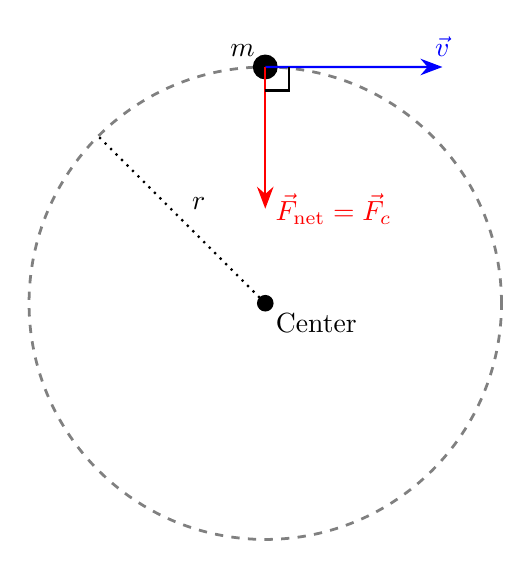
\begin{tikzpicture}[scale=1.5, line width=1pt]
        % 虚线圆周轨迹
        \draw[dashed, gray] (0,0) circle (2);
        \fill (0,0) circle (2pt) node[below right] {Center};
        
        % 物体
        \coordinate (Obj) at (0,2);
        \fill (Obj) circle (3pt) node[above left] {$m$};
        
        % 速度矢量 (切向)
        \draw[-{Stealth[scale=1.2]}, blue, thick] (Obj) -- (1.5,2) node[above] {$\vec{v}$};
        
        % 向心力矢量 (指向圆心)
        \draw[-{Stealth[scale=1.2]}, red, thick] (Obj) -- (0,0.8) node[right] {$\vec{F}_{\text{net}} = \vec{F}_c$};
        
        % 垂直符号
        \draw (0.2,2) -- (0.2, 1.8) -- (0, 1.8);
        
        % 半径虚线
        \draw[dotted, thick] (0,0) -- (135:2) node[midway, above right] {$r$};
    \end{tikzpicture}
    \caption{The net force $F_c$ is always perpendicular to the tangential velocity $\vec{v}$, pointing toward the center.}
\end{figure}


\subsection*{1.2 The "Role" Analogy}
A common misconception is that $F_c$ is a new type of physical force. In reality:
\begin{itemize}
    \item \textbf{Centripetal force is a requirement}, not a physical entity.
    \item It must be provided by actual forces such as Tension ($T$), Friction ($f$), Gravity ($F_g$), or Normal force ($F_N$).
\end{itemize}

\begin{figure}[h]
    \centering
    \begin{minipage}{0.45\textwidth}
        \centering
        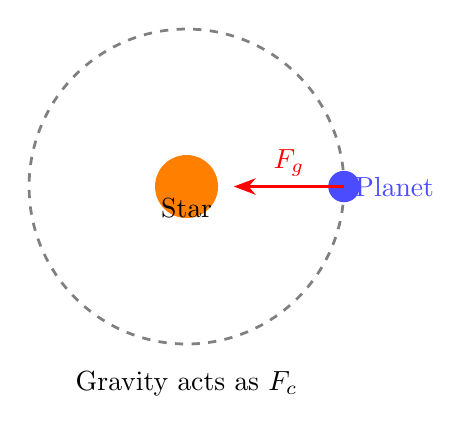
\begin{tikzpicture}[scale=1.0, line width=1pt]
            % 恒星与行星 (Gravity)
            \fill[orange] (0,0) circle (0.4) node[black, below=0.5] {Star};
            \draw[dashed, gray] (0,0) circle (2);
            \fill[blue!70!white] (2,0) circle (0.2) node[right=0.2] {Planet};
            
            % Fg 充当 Fc
            \draw[-{Stealth[scale=1.2]}, red, thick] (2,0) -- (0.6,0) node[midway, above] {$F_g$};
            \node at (0, -2.5) {Gravity acts as $F_c$};
        \end{tikzpicture}
    \end{minipage}%
    \hfill
    \begin{minipage}{0.45\textwidth}
        \centering
        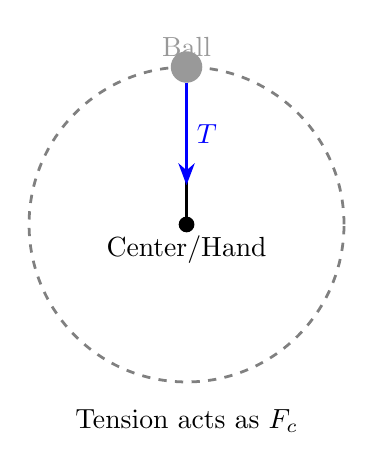
\begin{tikzpicture}[scale=1.0, line width=1pt]
            % 绳子与小球 (Tension)
            \fill (0,0) circle (0.1) node[below=0.1] {Center/Hand};
            \draw[dashed, gray] (0,0) circle (2);
            \fill[gray!80!white] (0,2) circle (0.2) node[above=0.1] {Ball};
            
            % 绳子
            \draw[thick] (0,0) -- (0,1.8);
            
            % T 充当 Fc
            \draw[-{Stealth[scale=1.2]}, blue, thick] (0,1.8) -- (0,0.5) node[midway, right] {$T$};
            \node at (0, -2.5) {Tension acts as $F_c$};
        \end{tikzpicture}
    \end{minipage}
    \caption{Centripetal force is not a new type of force, but a "role" fulfilled by real physical forces (such as $F_g$ or $T$).}
\end{figure}



\newpage

\section{Horizontal Circular Motion}

In these cases, we often ignore vertical motion as it is balanced ($F_N = mg$), and focus on the horizontal net force.

\subsection{Example 1: Car on a Flat Curve}


\begin{figure}[h]
    \centering
    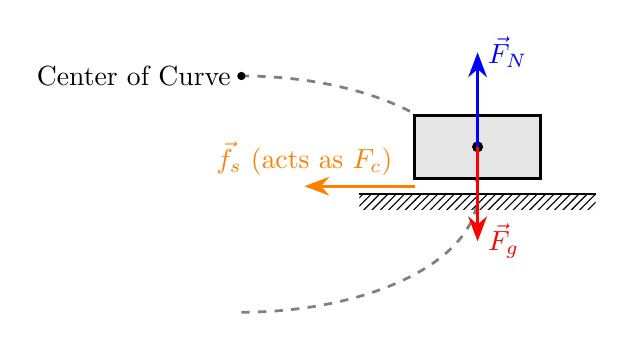
\begin{tikzpicture}[scale=1.0, line width=1pt]
        % 弯道圆心与轨迹参考线
        \draw[dashed, gray] (0, -2) arc (-90:90:3 and 1.5);
        \fill (0,1) circle (1.5pt) node[left] {Center of Curve};
        
        % 汽车后视图 (Rear View)
        \begin{scope}[shift={(3, -0.5)}]
            % 地面
            \draw[thick] (-1.5, 0) -- (1.5, 0);
            \fill[pattern=north east lines] (-1.5, -0.2) rectangle (1.5, 0);
            % 车身简化
            \draw[fill=gray!20] (-0.8, 0.2) rectangle (0.8, 1);
            \fill (0, 0.6) circle (2pt); % 质心
            
            % 受力图 (FBD)
            \draw[-{Stealth[scale=1.2]}, red] (0, 0.6) -- (0, -0.6) node[right] {$\vec{F}_g$};
            \draw[-{Stealth[scale=1.2]}, blue] (0, 0.6) -- (0, 1.8) node[right] {$\vec{F}_N$};
            % 摩擦力指向圆心
            \draw[-{Stealth[scale=1.2]}, orange] (-0.8, 0.1) -- (-2.2, 0.1) node[above] {$\vec{f}_s$ (acts as $F_c$)};
        \end{scope}
    \end{tikzpicture}
    \caption{Rear view of a car turning left. Static friction between the tires and the road provides the inward centripetal force.}
\end{figure}

For a car turning on a flat road, the \textbf{static friction} between the tires and the road provides the centripetal force.
\begin{equation*}
    f_s = \frac{mv^2}{r}
\end{equation*}
To avoid skidding, $f_s \leq \mu_s F_N$. Thus, the maximum safe speed is:
\begin{equation}
    v_{\text{max}} = \sqrt{\mu_s g r}
\end{equation}

\subsection{Example 2: Conical Pendulum}

\begin{figure}[h]
    \centering
    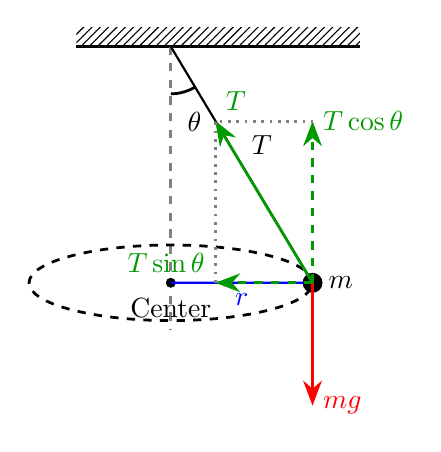
\begin{tikzpicture}[scale=1.2, line width=1pt]
        % 天花板
        \draw[thick] (-1, 2) -- (2, 2);
        \fill[pattern=north east lines] (-1, 2) rectangle (2, 2.2);
        
        % 竖直参考线
        \draw[dashed, gray] (0,2) -- (0,-1);
        
        % 小球和绳子
        \coordinate (Bob) at (1.5, -0.5);
        \draw[thick] (0,2) -- (Bob) node[midway, above right] {$T$};
        \fill (Bob) circle (3pt) node[right=2pt] {$m$};
        
        % 水平圆周轨迹
        \draw[dashed] (0,-0.5) ellipse (1.5 and 0.4);
        \fill (0,-0.5) circle (1.5pt) node[below=2pt] {Center};
        
        % 圆周半径
        \draw[thick, blue] (0,-0.5) -- (Bob) node[midway, below] {$r$};
        
        % 夹角 \theta
        \draw (0, 1.5) arc (270:301:0.5); 
        \node at (0.25, 1.2) {$\theta$};
        
        % 小球的受力分析分解 (FBD)
        \draw[-{Stealth[scale=1.2]}, red] (Bob) -- (1.5, -1.8) node[right] {$mg$};
        % 张力 T 矢量
        \draw[-{Stealth[scale=1.2]}, green!60!black] (Bob) -- ++(121:2) node[above right] {$T$};
        % T 的竖直分量
        \draw[dashed, green!60!black, -{Stealth[scale=1.2]}] (Bob) -- ++(0, 1.71) node[right] {$T\cos\theta$};
        % T 的水平方向分量(指向圆心)
        \draw[dashed, green!60!black, -{Stealth[scale=1.2]}] (Bob) -- ++(-1.03, 0) node[above left] {$T\sin\theta$};
        
        % 分解虚线框
        \draw[dotted, gray] (Bob) ++(-1.03, 0) -- ++(0, 1.71) -- ++(1.03, 0);
    \end{tikzpicture}
    \caption{A conical pendulum. The vertical component of tension balances gravity, while the horizontal component acts as the centripetal force.}
\end{figure}

A mass $m$ swings in a horizontal circle. The horizontal component of the tension ($T$) provides the centripetal force, while the vertical component balances gravity.
\begin{itemize}
    \item \textbf{Vertical:} $T\cos\theta = mg$
    \item \textbf{Horizontal:} $T\sin\theta = \frac{mv^2}{r}$
\end{itemize}



\newpage

\section{Vertical Circular Motion}

In vertical circles, gravity stays constant in direction (downward), but its contribution to the centripetal force changes depending on the object's position.

\subsection{Forces at the Top and Bottom}
Consider a bucket of water being swung in a vertical circle of radius $r$:

\begin{figure}[h]
    \centering
    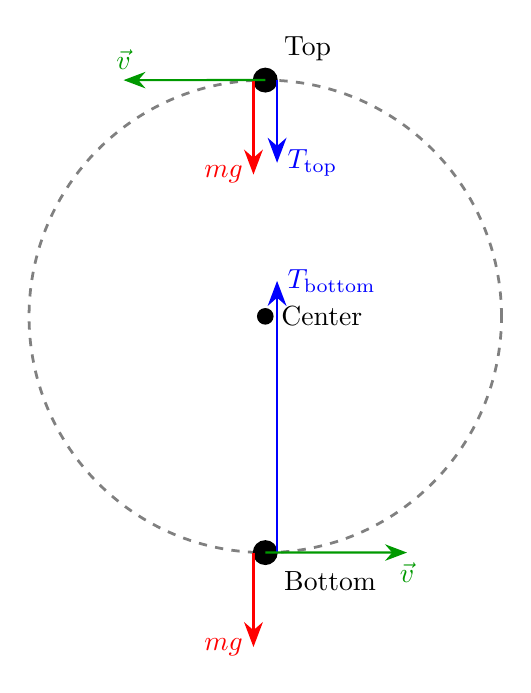
\begin{tikzpicture}[scale=1.5, line width=1pt]
        % 圆形轨迹
        \draw[dashed, gray] (0,0) circle (2);
        \fill (0,0) circle (2pt) node[right=2pt] {Center};
        
        % 最高点 (Top)
        \coordinate (Top) at (0,2);
        \fill (Top) circle (3pt) node[above right=3pt] {Top};
        
        % 最高点受力分析：重力和拉力同向，都指向圆心
        % mg 长度设为 0.8
        \draw[-{Stealth[scale=1.2]}, red] (-0.1, 2) -- (-0.1, 1.2) node[left] {$mg$};
        % T_top 较短，因为它只需要提供剩余的向心力 (假设总向心力需要 1.5, T_top = 0.7)
        \draw[-{Stealth[scale=1.2]}, blue] (0.1, 2) -- (0.1, 1.3) node[right] {$T_{\text{top}}$};
        % 切向速度
        \draw[thick, green!60!black, -{Stealth[scale=1.2]}] (Top) -- (-1.2, 2) node[above] {$\vec{v}$};
        
        % 最低点 (Bottom)
        \coordinate (Bot) at (0,-2);
        \fill (Bot) circle (3pt) node[below right=3pt] {Bottom};
        
        % 最低点受力分析：重力向下，拉力向上
        % mg 长度保持与上面相同的 0.8
        \draw[-{Stealth[scale=1.2]}, red] (-0.1, -2) -- (-0.1, -2.8) node[left] {$mg$};
        % T_bottom 必须非常长！(T_bot = 1.5 + 0.8 = 2.3)
        \draw[-{Stealth[scale=1.2]}, blue] (0.1, -2) -- (0.1, 0.3) node[right] {$T_{\text{bottom}}$};
        % 切向速度
        \draw[thick, green!60!black, -{Stealth[scale=1.2]}] (Bot) -- (1.2, -2) node[below] {$\vec{v}$};
    \end{tikzpicture}
    \caption{Forces at the top and bottom of a vertical circle. Notice the lengths of the tension vectors: $T_{\text{bottom}}$ must be drastically larger than $mg$ to provide a net inward force, whereas $T_{\text{top}}$ can be small because gravity "helps" pull inward.}
\end{figure}

\begin{enumerate}
    \item \textbf{At the Bottom:} Both Tension ($T$) and Gravity ($mg$) are on the same vertical line but in opposite directions.
    \begin{equation*}
        F_{\text{net}} = T_{\text{bottom}} - mg = \frac{mv^2}{r} \Rightarrow T_{\text{bottom}} = \frac{mv^2}{r} + mg
    \end{equation*}
    
    \item \textbf{At the Top:} Both Tension and Gravity point toward the center.
    \begin{equation*}
        F_{\text{net}} = T_{\text{top}} + mg = \frac{mv^2}{r} \Rightarrow T_{\text{top}} = \frac{mv^2}{r} - mg
    \end{equation*}
\end{enumerate}



\subsection{Critical Speed}
At the top of the circle, the "critical" case occurs when the string goes slack ($T_{\text{top}} = 0$). This is the minimum speed required to maintain the circle:
\begin{equation}
    0 + mg = \frac{mv^2}{r} \Rightarrow v_{\text{critical}} = \sqrt{gr}
\end{equation}

\section{Work and Energy in Circular Motion}

\begin{itemize}
    \item \textbf{Uniform Circular Motion:} Since $F_c$ is always perpendicular to the displacement ($\vec{v} \Delta t$), the work done by the centripetal force is \textbf{zero}.
    \begin{equation*}
        W = \vec{F}_c \cdot \Delta \vec{s} = F_c \Delta s \cos(90^\circ) = 0
    \end{equation*}
    \item \textbf{Consequence:} The kinetic energy (and thus the speed) of an object in UCM remains constant.
\end{itemize}

\end{document}